\subsection{测度空间上的淡拓扑}

设 X 为局部紧空间。在空间 \(\mathcal{M}(\mathrm{X};\mathbf{C})\) 上，可以考虑 \(\mathcal{K}(\mathrm{X};\mathbf{C})\) 中的逐点收敛拓扑，我们称之为 \(\mathcal{M}(\mathrm{X};\mathbf{C})\) 上的淡拓扑。

由于 \(\mathcal{K}(\mathrm{X};\mathbf{C}) = \mathcal{K}(\mathrm{X};\mathbf{R}) + i\mathcal{K}(\mathrm{X};\mathbf{R})\)，\(\mathcal{M}(\mathrm{X};\mathbf{C})\) 上的淡拓扑由半范数 \(\sup_{1\leqslant i\leqslant n}|\mu (f_i)|\) 确定，其中 \((f_i)_{1\leqslant i\leqslant n}\) 是 \(\mathcal{K}(\mathrm{X};\mathbf{R})\) （或 \(\mathcal{K}_{+}(\mathrm{X})\) ）中函数的任意有限序列。说 \(\mathfrak{F}\) （\(\mathcal{M}(\mathrm{X};\mathbf{C})\) 上的滤子）淡收敛于测度 \(\mu_0\)，就意味着

\[
\mu_ {0} (f) = \lim _ {\mu , \mathfrak {F}} \mu (f)
\]

对每个函数 \(f \in \mathcal{K}(\mathrm{X};\mathbf{R})\) 成立。对每个函数 \(f \in \mathcal{K}(\mathrm{X};\mathbf{C})\)，映射 \(\mu \mapsto \mu(f)\) 是空间 \(\mathcal{M}(\mathrm{X};\mathbf{C})\) 上的淡连续线性形式。

命题 13. --- 设 X 为局部紧空间，且对每个 \(x \in X\)，设 \(\varepsilon_{x}\) 为点 x 处的 Dirac 测度。映射 \(x \mapsto \varepsilon_{x}\) 是 X 到装备淡拓扑的测度空间 \(\mathcal{M}(\mathrm{X};\mathbf{C})\) 的一个子空间上的同胚。此外，若以 \(X'\) 表示把无穷远点 \(\omega\) 添加到 X 上所得的紧空间，则 \(\varepsilon_{x}\) 当 x 趋于 \(\omega\) 时趋于 0。

对每个函数 \(f \in \mathcal{K}(\mathrm{X};\mathbf{C})\)，有 \(\langle f,\varepsilon_x\rangle = f(x)\)；由于 \(f\) 连续，这就证明映射 \(x \mapsto \varepsilon_x\) 连续。若 \(x,y\) 是 \(\mathbf{X}\) 的两个不同点，则存在函数 \(f \in \mathcal{K}(\mathrm{X};\mathbf{C})\) 使 \(f(x) = 1\)，\(f(y) = 0\)（No. 2, 引理 1），这就证明 \(\varepsilon_x \neq \varepsilon_y\)；因而映射 \(x \mapsto \varepsilon_x\) 是单射。此外，对每个函数 \(f \in \mathcal{K}(\mathrm{X};\mathbf{C})\)，按定义，\(\langle f,\varepsilon_x\rangle\) 当 \(x\) 趋于 \(\omega\) 时趋于 0，因此 \(x \mapsto \varepsilon_x\) 可连续延拓到 \(X' = X \cup \{\omega\}\) ，方法是在点 \(\omega\) 处赋予它值 0。这个延拓后的映射也是单射，因为 \(\varepsilon_x \neq 0\) 对所有 \(x \in X\) 成立。于是它是紧空间 \(X'\) 到 \(\mathcal{M}(\mathrm{X};\mathbf{C})\) 的一个子空间上的同胚，因为 \(\mathcal{M}(\mathrm{X};\mathbf{C})\) 对淡拓扑是 Hausdorff 的（GT, I, §9, No. 4, Th. 2 的推论 2）。

命题 14. --- 在空间 \(\mathcal{M}(\mathrm{X};\mathbf{C})\) （局部紧空间 \(\mathbf{X}\) 上的测度所成的空间）中，正测度所成的锥 \(\mathcal{M}_{+}(\mathbf{X})\) 对于由淡拓扑导出的一致结构是完备的（从而在 \(\mathcal{M}(\mathrm{X};\mathbf{C})\) 中是淡闭的）。

事实上，考虑一个 Cauchy 滤子 \(\Phi\)（关于 \(\mathcal{M}_{+}(\mathrm{X})\) 上的淡一致结构）；按定义，极限 \(\mu_{0}(f) = \lim_{\mu,\Phi} \mu(f)\) 对每个函数 \(f \in \mathcal{K}(\mathrm{X}; \mathbf{C})\) 存在，且由不等式延拓原理，\(\mu_{0}(f) \geqslant 0\) 对每个函数 \(f \in \mathcal{K}_{+}(\mathrm{X})\) 成立；由此推出 \(\mu_{0}\) 是 X 上的正测度（No. 5, Th. 1）。

\pandocbounded{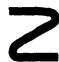
\includegraphics[keepaspectratio]{images/part001_58cd264b.jpg}}

应当注意，空间 \(\mathcal{M}(\mathrm{X};\mathbf{C})\) （或 \(\mathcal{M}(\mathrm{X};\mathbf{R})\) ）本身对淡一致结构不必是完备的（TVS, II, §6, No. 7）。

推论. --- 若 A 与 B 是 \(\mathcal{M}_{+}(\mathrm{X})\) 的两个淡闭子集，则 \(A + B\) 在 \(\mathcal{M}_{+}(\mathrm{X})\) 中淡闭（从而在 \(\mathcal{M}(\mathrm{X};\mathbf{C})\) 中也淡闭）。

这实际上是局部凸空间中弱完备的带顶点凸锥的一个一般性质（TVS, II, §6, No. 8, Prop. 11 的推论 2）。

命题 15. --- 设 H 为 \(\mathcal{M}(\mathrm{X};\mathbf{C})\) 的一个子集。下列性质等价：

\begin{enumerate}
\def\labelenumi{\alph{enumi})}
\item
  H 是淡有界的。
\item
  H 是淡相对紧的。
\item
  H 是等度连续的。
\item
  对 X 的每个紧子集 K，存在数 \(M_{K} \geqslant 0\)，使 \(|\mu(f)| \leqslant M_{K}\|f\|\) 对每个测度 \(\mu \in H\) 和每个函数 \(f \in \mathcal{K}(X, K; \mathbf{C})\) 成立。
\end{enumerate}

由于 \(\mathcal{K}(\mathrm{X};\mathbf{C})\) 是桶式空间（No. 1, Prop. 2），性质 a)、b) 与 c) 的等价性由 TVS, III, §4, No. 1 的 Scholium 得出。

显然 d) 蕴含 a)。最后，若 H 等度连续，则测度 \(\mu\in H\) 在 \(\mathcal{K}(X,K;\mathbf{C})\) 上的限制所成的集合也等度连续，由此得到条件 d)，因为 \(\mathcal{K}(X,K;\mathbf{C})\) 是赋范空间。

* 我们将在第 IV 章 §4 No. 6 中看到，命题 15 的诸条件也等价于如下条件：对 X 的每个紧子集 K，存在常数 \(\mathrm{M}_{\mathrm{K}}\)，使 \(|\mu|(\mathrm{K}) \leqslant \mathrm{M}_{\mathrm{K}}\) 对每个测度 \(\mu \in \mathrm{H}\) 成立。

推论 1. --- 设 \(\nu\) 为 X 上的正测度；测度 \(\mu\) （满足 \(|\mu| \leqslant \nu\) 的那些）所成的集合是淡紧的。

推论 2. --- 测度 \(\mu\) （满足 \(\|\mu\| \leqslant a\) ，其中 a 为任意有限数 \(>0\) ）所成的集合是淡紧的。

推论 3. --- 若 X 是紧的，则 X 上的正测度 \(\mu\) （满足 \(\|\mu\| = 1\) 的那些）所成的集合是淡紧的。

事实上，它是使 \(\|\mu\|\leqslant1\) 的测度所成的淡紧集（推论 2）与分别由关系式 \(\mu\geqslant0\) 和 \(\mu(1)=1\) 所确定的淡闭集的交（No. 8, Prop. 10 的推论 2）。

推论 4. --- 在空间 \(\mathcal{M}(\mathrm{X};\mathbf{C})\) 中，映射 \(\mu \mapsto \| \mu \|\) 对淡拓扑是下半连续的。

这是推论 2 的直接结果。

\pandocbounded{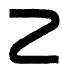
\includegraphics[keepaspectratio]{images/part001_13b41992.jpg}}

应当注意，映射 \(\mu \mapsto |\mu|\) （\(\mathcal{M}(\mathrm{X};\mathbf{C})\) 到自身的映射）对淡拓扑不必是连续的（习题 9）。

命题 16. --- 设 K 为 X 的紧子集，H 为 \(\mathcal{M}(\mathrm{X};\mathbf{C})\) 的淡有界子集；则双线性型 \((f,\mu)\mapsto\langle f,\mu\rangle\) 在 \(\mathcal{K}(\mathrm{X},\mathrm{K};\mathbf{C})\times\mathrm{H}\) 上连续，这里 \(\mathcal{K}(\mathrm{X},\mathrm{K};\mathbf{C})\) 装备一致收敛拓扑，而 H 装备淡拓扑。

事实上，存在数 \(M \geqslant 0\)，使得

\[
| \mu (f) | \leqslant \mathrm{M} \| f \|
\]

对每个函数 \(f \in \mathcal{K}(\mathrm{X},\mathrm{K};\mathbf{C})\) 和每个测度 \(\mu \in \mathrm{H}\) 成立（命题 15）。若 \(\mu_0\) 与 \(\mu\) 是属于 \(\mathrm{H}\) 的两个测度，\(f_0\) 与 \(f\) 是 \(\mathcal{K}(\mathrm{X},\mathrm{K};\mathbf{C})\) 中的两个函数，则

\[
\begin{array}{r l} | \mu (f) - \mu_ {0} (f _ {0}) | & = | \mu (f - f _ {0}) + \mu (f _ {0}) - \mu_ {0} (f _ {0}) | \\ & \leqslant \mathrm{M} \| f - f _ {0} \| + | \mu (f _ {0}) - \mu_ {0} (f _ {0}) |, \end{array}
\]

而当 \(\|f-f_{0}\|\) 与 \(|\mu(f_{0})-\mu_{0}(f_{0})|\) 任意小时，最后一个量也任意小，这就证明了命题。
% semantic-fragments: legacy-input-seam
\relax{}
